% Options for packages loaded elsewhere
\PassOptionsToPackage{unicode}{hyperref}
\PassOptionsToPackage{hyphens}{url}
%
\documentclass[
  twocolumn]{article}
\usepackage{lmodern}
\usepackage{amssymb,amsmath}
\usepackage{ifxetex,ifluatex}
\ifnum 0\ifxetex 1\fi\ifluatex 1\fi=0 % if pdftex
  \usepackage[T1]{fontenc}
  \usepackage[utf8]{inputenc}
  \usepackage{textcomp} % provide euro and other symbols
\else % if luatex or xetex
  \usepackage{unicode-math}
  \defaultfontfeatures{Scale=MatchLowercase}
  \defaultfontfeatures[\rmfamily]{Ligatures=TeX,Scale=1}
\fi
% Use upquote if available, for straight quotes in verbatim environments
\IfFileExists{upquote.sty}{\usepackage{upquote}}{}
\IfFileExists{microtype.sty}{% use microtype if available
  \usepackage[]{microtype}
  \UseMicrotypeSet[protrusion]{basicmath} % disable protrusion for tt fonts
}{}
\makeatletter
\@ifundefined{KOMAClassName}{% if non-KOMA class
  \IfFileExists{parskip.sty}{%
    \usepackage{parskip}
  }{% else
    \setlength{\parindent}{0pt}
    \setlength{\parskip}{6pt plus 2pt minus 1pt}}
}{% if KOMA class
  \KOMAoptions{parskip=half}}
\makeatother
\usepackage{xcolor}
\IfFileExists{xurl.sty}{\usepackage{xurl}}{} % add URL line breaks if available
\IfFileExists{bookmark.sty}{\usepackage{bookmark}}{\usepackage{hyperref}}
\hypersetup{
  pdftitle={Report DOPP Exercise 3},
  pdfauthor={Helmuth Breitenfellner, 8725866; László Király, 9227679; Lukas Steindl, 11743494; Gerald Weber, 0125536},
  hidelinks,
  pdfcreator={LaTeX via pandoc}}
\urlstyle{same} % disable monospaced font for URLs
\usepackage[margin=1in]{geometry}
\usepackage{graphicx,grffile}
\makeatletter
\def\maxwidth{\ifdim\Gin@nat@width>\linewidth\linewidth\else\Gin@nat@width\fi}
\def\maxheight{\ifdim\Gin@nat@height>\textheight\textheight\else\Gin@nat@height\fi}
\makeatother
% Scale images if necessary, so that they will not overflow the page
% margins by default, and it is still possible to overwrite the defaults
% using explicit options in \includegraphics[width, height, ...]{}
\setkeys{Gin}{width=\maxwidth,height=\maxheight,keepaspectratio}
% Set default figure placement to htbp
\makeatletter
\def\fps@figure{htbp}
\makeatother
\setlength{\emergencystretch}{3em} % prevent overfull lines
\providecommand{\tightlist}{%
  \setlength{\itemsep}{0pt}\setlength{\parskip}{0pt}}
\setcounter{secnumdepth}{-\maxdimen} % remove section numbering

\title{Report DOPP Exercise 3}
\usepackage{etoolbox}
\makeatletter
\providecommand{\subtitle}[1]{% add subtitle to \maketitle
  \apptocmd{\@title}{\par {\large #1 \par}}{}{}
}
\makeatother
\subtitle{Topic 16 - Change of City Quality of Life Rankings over Time}
\author{Helmuth Breitenfellner, 8725866 \and László Király, 9227679 \and Lukas Steindl, 11743494 \and Gerald Weber, 0125536}
\date{2020-01-27}

\begin{document}
\maketitle

\hypertarget{executive-summary}{%
\section{Executive Summary}\label{executive-summary}}

We have been analysing data for various city and country rankings and
indices, measuring overall quality of living (QoL). These data were
merged with additional statistics for cities and countries related to
health, environmental and economical situation. The main focus was on
the ranking published by Mercer, ranking and indices published by Numbeo
and statistics published by WHO, the United Nations, and other data
collected by Gap Minder.

Our goal was to answer the questions:

\begin{itemize}
\tightlist
\item
  How do the rankings change over time?
\item
  How do these rankings correlate with each other for one specific year?
\item
  How do they correlate with other statistics about the countries in
  which the cities are located?
\item
  How do they correlate with quality of living rankings of the country
  in which the cities are located?
\item
  What are the determining characteristics for livability of a city? How
  do they correlate with cost of living?
\end{itemize}

We found that the quality of living indices are going upwards - except
for the last three years where there is an small downwards trend
visible. Here one should also understand that the methodology of the
rankings and indexes used is continuously adjusted.

There is a strong correlation between the rankings published by Mercer
and the one calculated by Numbeo. Other city rankings (e.g.~UN Habitat
ranking) do not correlate so well.

The correlation of country-level statistics (e.g.~GDP per capita,
emission damage, health care system) to the city-level QoL ranking
turned out to be surprisingly high. Almost 50\% of the variance of the
QoL index can be explained by country-level statistics.

Similarly, the correlation with country-level QoL rankings (e.g.~the
Numbeo country ranking) is again very high. We looked into cities which
are not following the country trend, like Mumbai (vastly exceeding the
QoL of India) and Rome (much lower QoL as Italy).

We found that the three major characteristics determining the livability
of a city (according to these QoL rankings) are health care, cost of
living and purchasing power. On the other hand the QoL rankings suffer
from high pollution rates, high property-to-income-ratios and long
commute times (inefficient traffic).

\hypertarget{questions-answered}{%
\section{Questions answered}\label{questions-answered}}

\hypertarget{change-of-qol-rankings-and-indices-over-time}{%
\subsection{Change of QoL Rankings and Indices over
Time}\label{change-of-qol-rankings-and-indices-over-time}}

The following plot shows the average index values over time for the
Quality of Live (QoL) identified by Numbeo, together with the components
which influence this index.

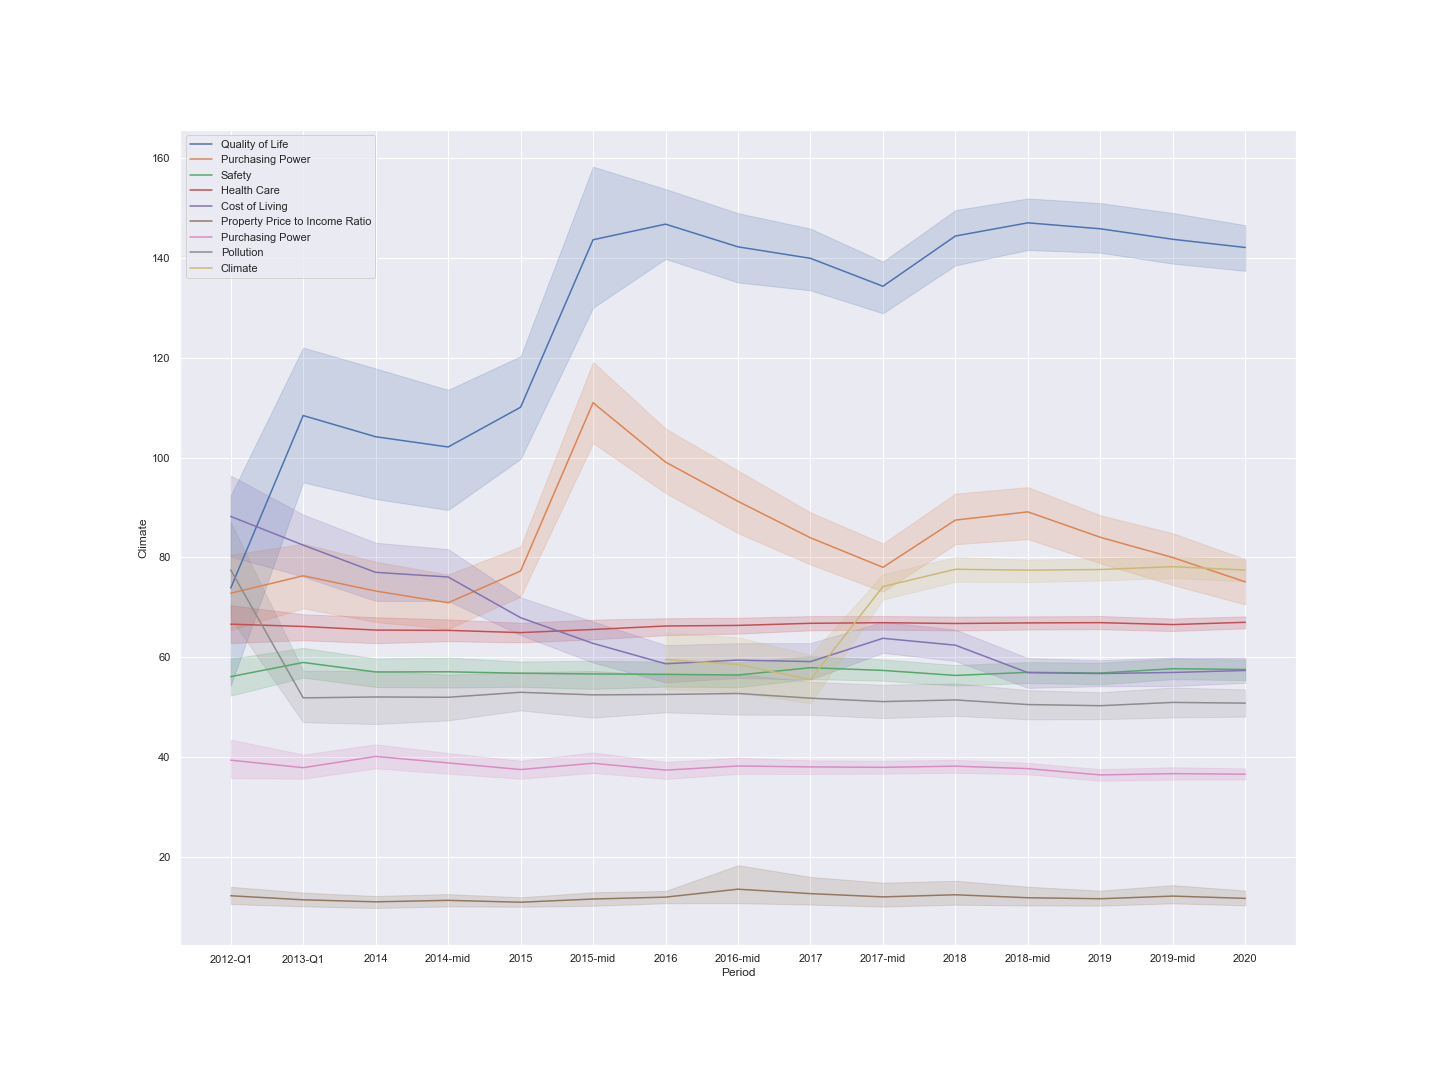
\includegraphics[width=1\linewidth]{visuals/RankingsOverTime}

\hypertarget{correlation-of-city-qol-rankings-with-each-other}{%
\subsection{Correlation of City QoL Rankings with each
other}\label{correlation-of-city-qol-rankings-with-each-other}}

With this plot we investigated the correlation of the rankings
identified by Numbeo with those identified by Mercer as well as the UN
Habitat data, specifically looking into the year 2012 (where the most
data was available).

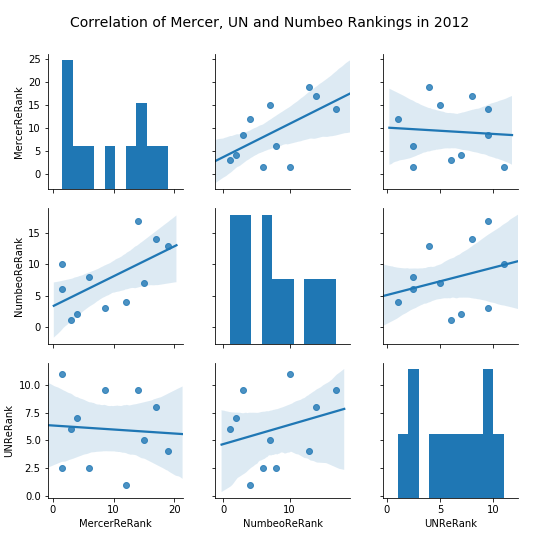
\includegraphics[width=1\linewidth]{visuals/CorrelationOfMercerAndUNAndNumbeoRanking2012}

The correlation between Numbeo and Mercer is very clearly visible; the
correlation to the UN Habitat ranking however is lower.

\hypertarget{correlation-of-city-qol-rankings-with-country-statistics}{%
\subsection{Correlation of City QoL Rankings with Country
Statistics}\label{correlation-of-city-qol-rankings-with-country-statistics}}

We looked into the correlation of health-related, economical and
environmental statistics of countries and their influence on the Quality
of Living for their cities.

As an example here a plot of the correlation between GDP per capita
(purchase-power adjusted) and QoL:

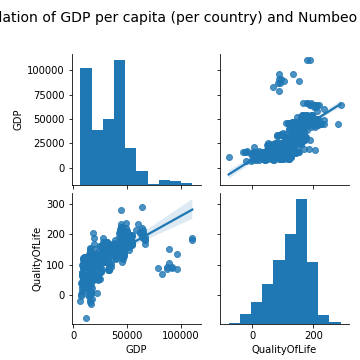
\includegraphics[width=1\linewidth]{visuals/CorrelationGDP_QoL}

\hypertarget{correlation-of-city-qol-rankings-with-country-qol-rankings}{%
\subsection{Correlation of City QoL Rankings with Country QoL
Rankings}\label{correlation-of-city-qol-rankings-with-country-qol-rankings}}

\hypertarget{determining-factors-for-city-qol}{%
\subsection{Determining Factors for City
QoL}\label{determining-factors-for-city-qol}}

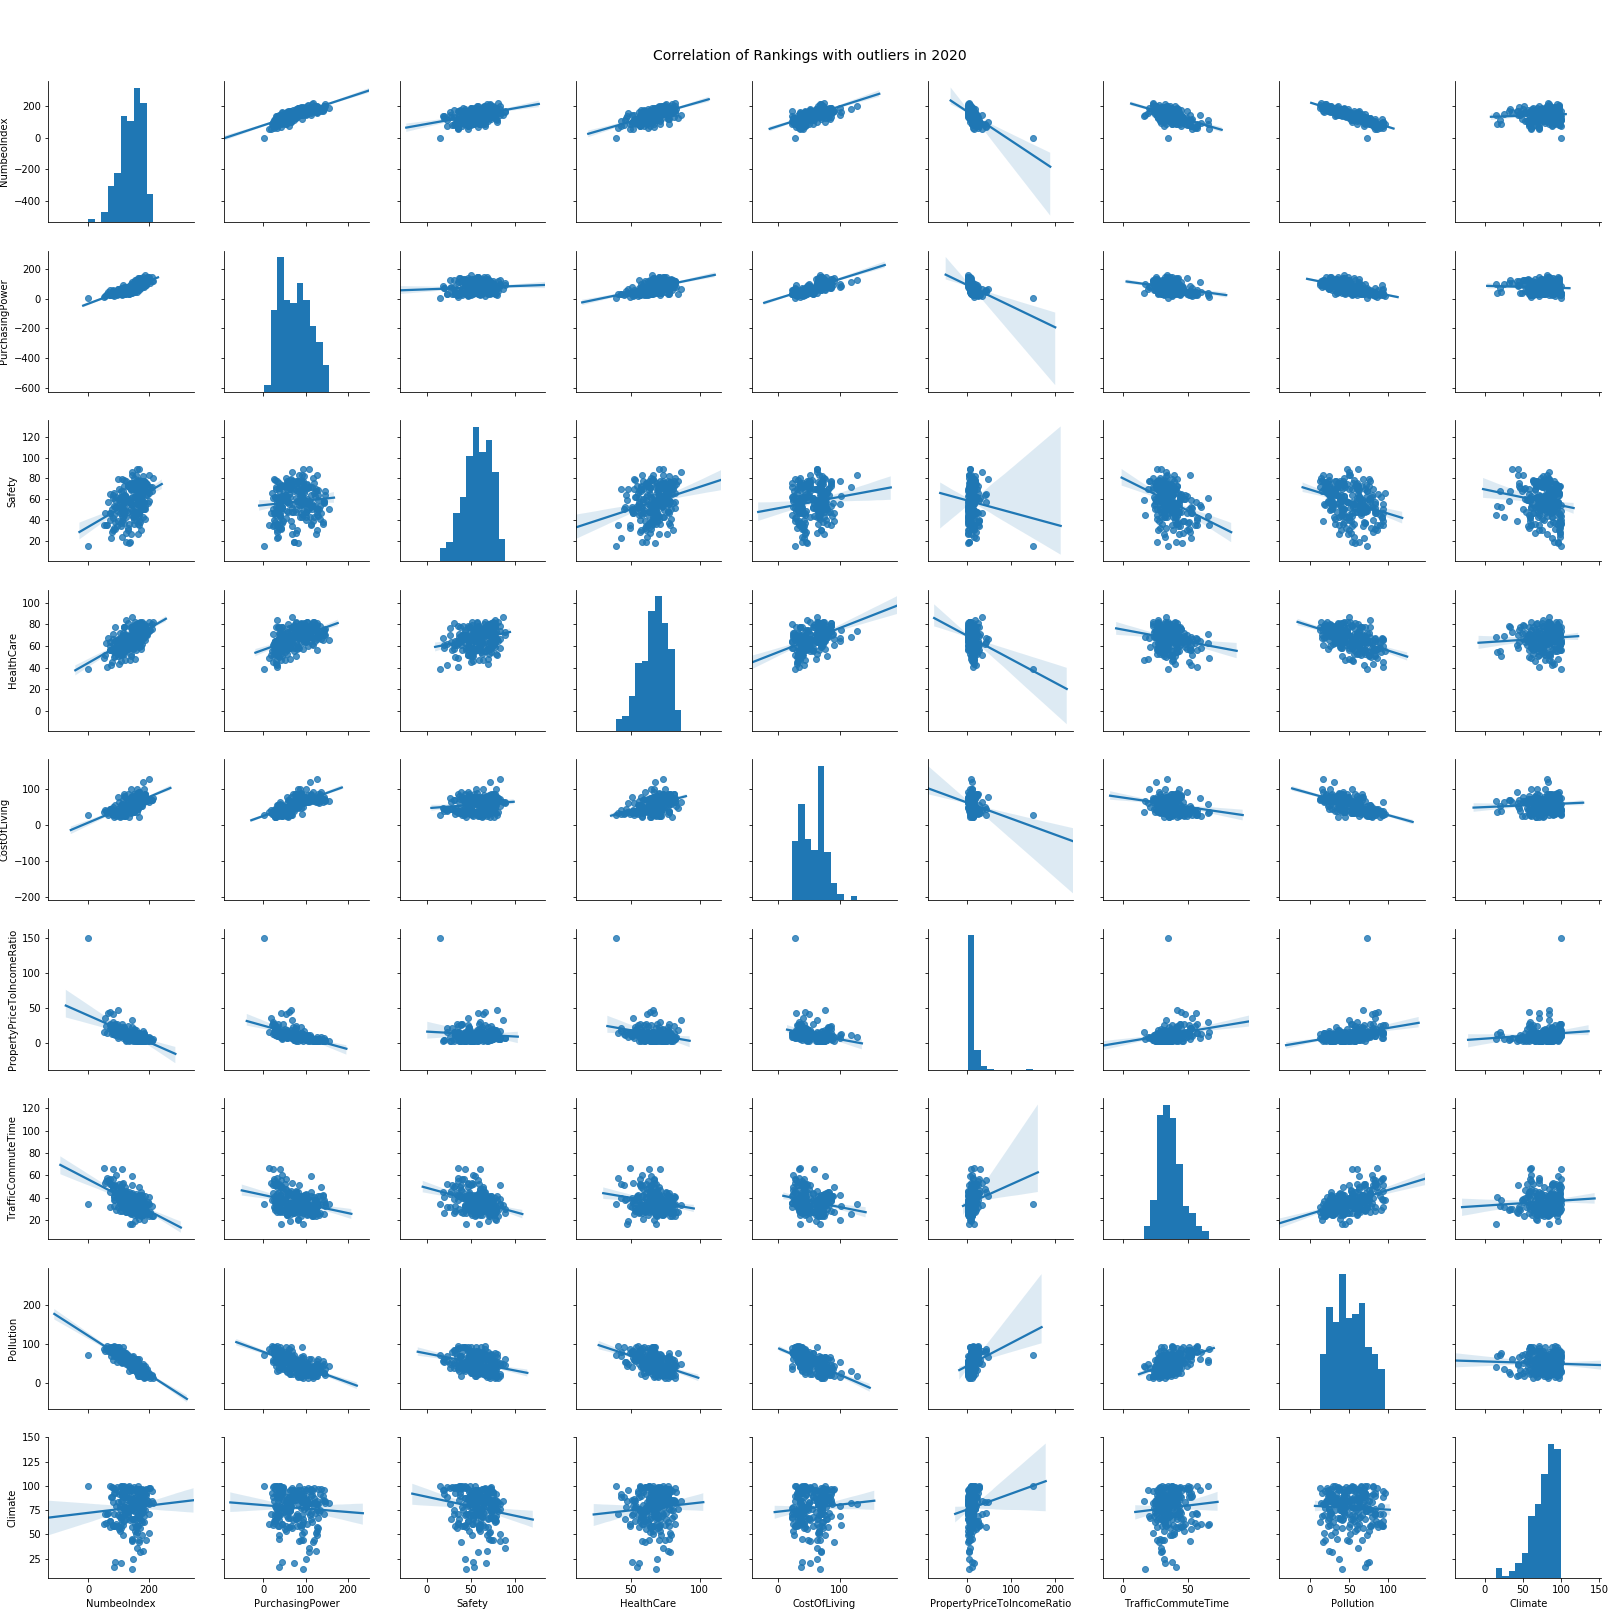
\includegraphics[width=1\linewidth]{visuals/CorrelationOfRankingsIn2020WithOutliers}

\hypertarget{correlation-of-cost-of-living-with-other-city-characteristics.}{%
\subsection{Correlation of Cost of Living with other
city-characteristics.}\label{correlation-of-cost-of-living-with-other-city-characteristics.}}

Purchasing Power and Healthcare are indicators that the cost of living
will also be high.

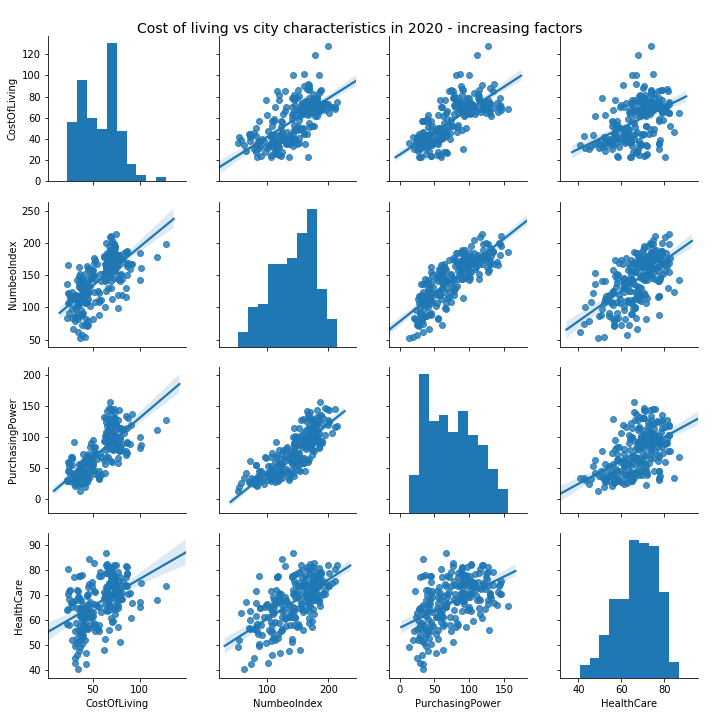
\includegraphics[width=1\linewidth]{visuals/CostOfLivingCorrelationIn2020}

Pollution, inefficient traffic, and a high
property-price-to-income-ratio (pptir) reduce the cost of living index.

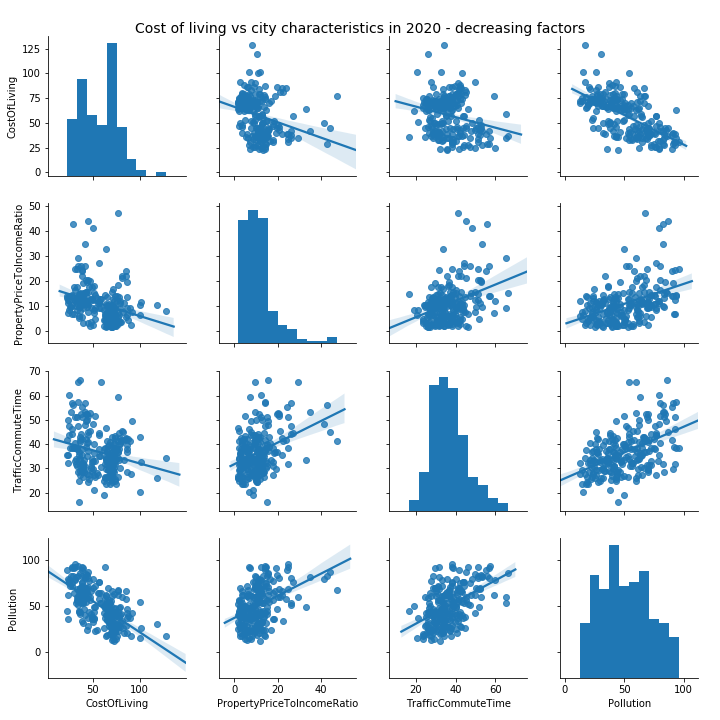
\includegraphics[width=1\linewidth]{visuals/CostOfLivingCorrelationIn2020NegativeInfluencers}

The pptir is an indication on how long an average family has to work to
buy an average property(house/flat) in a city. It is interesting to see
that there is a negative correlation between this indicator and the cost
of. It may seem counterintuitive that it is easier to buy a house when
the cost of living is higher.

\end{document}
